% Options for packages loaded elsewhere
% Options for packages loaded elsewhere
\PassOptionsToPackage{unicode}{hyperref}
\PassOptionsToPackage{hyphens}{url}
\PassOptionsToPackage{dvipsnames,svgnames,x11names}{xcolor}
%
\documentclass[
  letterpaper,
]{article}
\usepackage{xcolor}
\usepackage[top=20mm,left=20mm,right=20mm,bottom=20mm]{geometry}
\usepackage{amsmath,amssymb}
\setcounter{secnumdepth}{5}
\usepackage{iftex}
\ifPDFTeX
  \usepackage[T1]{fontenc}
  \usepackage[utf8]{inputenc}
  \usepackage{textcomp} % provide euro and other symbols
\else % if luatex or xetex
  \usepackage{unicode-math} % this also loads fontspec
  \defaultfontfeatures{Scale=MatchLowercase}
  \defaultfontfeatures[\rmfamily]{Ligatures=TeX,Scale=1}
\fi
\usepackage{lmodern}
\ifPDFTeX\else
  % xetex/luatex font selection
\fi
% Use upquote if available, for straight quotes in verbatim environments
\IfFileExists{upquote.sty}{\usepackage{upquote}}{}
\IfFileExists{microtype.sty}{% use microtype if available
  \usepackage[]{microtype}
  \UseMicrotypeSet[protrusion]{basicmath} % disable protrusion for tt fonts
}{}
\makeatletter
\@ifundefined{KOMAClassName}{% if non-KOMA class
  \IfFileExists{parskip.sty}{%
    \usepackage{parskip}
  }{% else
    \setlength{\parindent}{0pt}
    \setlength{\parskip}{6pt plus 2pt minus 1pt}}
}{% if KOMA class
  \KOMAoptions{parskip=half}}
\makeatother
% Make \paragraph and \subparagraph free-standing
\makeatletter
\ifx\paragraph\undefined\else
  \let\oldparagraph\paragraph
  \renewcommand{\paragraph}{
    \@ifstar
      \xxxParagraphStar
      \xxxParagraphNoStar
  }
  \newcommand{\xxxParagraphStar}[1]{\oldparagraph*{#1}\mbox{}}
  \newcommand{\xxxParagraphNoStar}[1]{\oldparagraph{#1}\mbox{}}
\fi
\ifx\subparagraph\undefined\else
  \let\oldsubparagraph\subparagraph
  \renewcommand{\subparagraph}{
    \@ifstar
      \xxxSubParagraphStar
      \xxxSubParagraphNoStar
  }
  \newcommand{\xxxSubParagraphStar}[1]{\oldsubparagraph*{#1}\mbox{}}
  \newcommand{\xxxSubParagraphNoStar}[1]{\oldsubparagraph{#1}\mbox{}}
\fi
\makeatother

\usepackage{color}
\usepackage{fancyvrb}
\newcommand{\VerbBar}{|}
\newcommand{\VERB}{\Verb[commandchars=\\\{\}]}
\DefineVerbatimEnvironment{Highlighting}{Verbatim}{commandchars=\\\{\}}
% Add ',fontsize=\small' for more characters per line
\usepackage{framed}
\definecolor{shadecolor}{RGB}{241,243,245}
\newenvironment{Shaded}{\begin{snugshade}}{\end{snugshade}}
\newcommand{\AlertTok}[1]{\textcolor[rgb]{0.68,0.00,0.00}{#1}}
\newcommand{\AnnotationTok}[1]{\textcolor[rgb]{0.37,0.37,0.37}{#1}}
\newcommand{\AttributeTok}[1]{\textcolor[rgb]{0.40,0.45,0.13}{#1}}
\newcommand{\BaseNTok}[1]{\textcolor[rgb]{0.68,0.00,0.00}{#1}}
\newcommand{\BuiltInTok}[1]{\textcolor[rgb]{0.00,0.23,0.31}{#1}}
\newcommand{\CharTok}[1]{\textcolor[rgb]{0.13,0.47,0.30}{#1}}
\newcommand{\CommentTok}[1]{\textcolor[rgb]{0.37,0.37,0.37}{#1}}
\newcommand{\CommentVarTok}[1]{\textcolor[rgb]{0.37,0.37,0.37}{\textit{#1}}}
\newcommand{\ConstantTok}[1]{\textcolor[rgb]{0.56,0.35,0.01}{#1}}
\newcommand{\ControlFlowTok}[1]{\textcolor[rgb]{0.00,0.23,0.31}{\textbf{#1}}}
\newcommand{\DataTypeTok}[1]{\textcolor[rgb]{0.68,0.00,0.00}{#1}}
\newcommand{\DecValTok}[1]{\textcolor[rgb]{0.68,0.00,0.00}{#1}}
\newcommand{\DocumentationTok}[1]{\textcolor[rgb]{0.37,0.37,0.37}{\textit{#1}}}
\newcommand{\ErrorTok}[1]{\textcolor[rgb]{0.68,0.00,0.00}{#1}}
\newcommand{\ExtensionTok}[1]{\textcolor[rgb]{0.00,0.23,0.31}{#1}}
\newcommand{\FloatTok}[1]{\textcolor[rgb]{0.68,0.00,0.00}{#1}}
\newcommand{\FunctionTok}[1]{\textcolor[rgb]{0.28,0.35,0.67}{#1}}
\newcommand{\ImportTok}[1]{\textcolor[rgb]{0.00,0.46,0.62}{#1}}
\newcommand{\InformationTok}[1]{\textcolor[rgb]{0.37,0.37,0.37}{#1}}
\newcommand{\KeywordTok}[1]{\textcolor[rgb]{0.00,0.23,0.31}{\textbf{#1}}}
\newcommand{\NormalTok}[1]{\textcolor[rgb]{0.00,0.23,0.31}{#1}}
\newcommand{\OperatorTok}[1]{\textcolor[rgb]{0.37,0.37,0.37}{#1}}
\newcommand{\OtherTok}[1]{\textcolor[rgb]{0.00,0.23,0.31}{#1}}
\newcommand{\PreprocessorTok}[1]{\textcolor[rgb]{0.68,0.00,0.00}{#1}}
\newcommand{\RegionMarkerTok}[1]{\textcolor[rgb]{0.00,0.23,0.31}{#1}}
\newcommand{\SpecialCharTok}[1]{\textcolor[rgb]{0.37,0.37,0.37}{#1}}
\newcommand{\SpecialStringTok}[1]{\textcolor[rgb]{0.13,0.47,0.30}{#1}}
\newcommand{\StringTok}[1]{\textcolor[rgb]{0.13,0.47,0.30}{#1}}
\newcommand{\VariableTok}[1]{\textcolor[rgb]{0.07,0.07,0.07}{#1}}
\newcommand{\VerbatimStringTok}[1]{\textcolor[rgb]{0.13,0.47,0.30}{#1}}
\newcommand{\WarningTok}[1]{\textcolor[rgb]{0.37,0.37,0.37}{\textit{#1}}}

\usepackage{longtable,booktabs,array}
\usepackage{calc} % for calculating minipage widths
% Correct order of tables after \paragraph or \subparagraph
\usepackage{etoolbox}
\makeatletter
\patchcmd\longtable{\par}{\if@noskipsec\mbox{}\fi\par}{}{}
\makeatother
% Allow footnotes in longtable head/foot
\IfFileExists{footnotehyper.sty}{\usepackage{footnotehyper}}{\usepackage{footnote}}
\makesavenoteenv{longtable}
\usepackage{graphicx}
\makeatletter
\newsavebox\pandoc@box
\newcommand*\pandocbounded[1]{% scales image to fit in text height/width
  \sbox\pandoc@box{#1}%
  \Gscale@div\@tempa{\textheight}{\dimexpr\ht\pandoc@box+\dp\pandoc@box\relax}%
  \Gscale@div\@tempb{\linewidth}{\wd\pandoc@box}%
  \ifdim\@tempb\p@<\@tempa\p@\let\@tempa\@tempb\fi% select the smaller of both
  \ifdim\@tempa\p@<\p@\scalebox{\@tempa}{\usebox\pandoc@box}%
  \else\usebox{\pandoc@box}%
  \fi%
}
% Set default figure placement to htbp
\def\fps@figure{htbp}
\makeatother





\setlength{\emergencystretch}{3em} % prevent overfull lines

\providecommand{\tightlist}{%
  \setlength{\itemsep}{0pt}\setlength{\parskip}{0pt}}



 


\makeatletter
\@ifpackageloaded{tcolorbox}{}{\usepackage[skins,breakable]{tcolorbox}}
\@ifpackageloaded{fontawesome5}{}{\usepackage{fontawesome5}}
\definecolor{quarto-callout-color}{HTML}{909090}
\definecolor{quarto-callout-note-color}{HTML}{0758E5}
\definecolor{quarto-callout-important-color}{HTML}{CC1914}
\definecolor{quarto-callout-warning-color}{HTML}{EB9113}
\definecolor{quarto-callout-tip-color}{HTML}{00A047}
\definecolor{quarto-callout-caution-color}{HTML}{FC5300}
\definecolor{quarto-callout-color-frame}{HTML}{acacac}
\definecolor{quarto-callout-note-color-frame}{HTML}{4582ec}
\definecolor{quarto-callout-important-color-frame}{HTML}{d9534f}
\definecolor{quarto-callout-warning-color-frame}{HTML}{f0ad4e}
\definecolor{quarto-callout-tip-color-frame}{HTML}{02b875}
\definecolor{quarto-callout-caution-color-frame}{HTML}{fd7e14}
\makeatother
\makeatletter
\@ifpackageloaded{caption}{}{\usepackage{caption}}
\AtBeginDocument{%
\ifdefined\contentsname
  \renewcommand*\contentsname{Table of contents}
\else
  \newcommand\contentsname{Table of contents}
\fi
\ifdefined\listfigurename
  \renewcommand*\listfigurename{List of Figures}
\else
  \newcommand\listfigurename{List of Figures}
\fi
\ifdefined\listtablename
  \renewcommand*\listtablename{List of Tables}
\else
  \newcommand\listtablename{List of Tables}
\fi
\ifdefined\figurename
  \renewcommand*\figurename{Figure}
\else
  \newcommand\figurename{Figure}
\fi
\ifdefined\tablename
  \renewcommand*\tablename{Table}
\else
  \newcommand\tablename{Table}
\fi
}
\@ifpackageloaded{float}{}{\usepackage{float}}
\floatstyle{ruled}
\@ifundefined{c@chapter}{\newfloat{codelisting}{h}{lop}}{\newfloat{codelisting}{h}{lop}[chapter]}
\floatname{codelisting}{Listing}
\newcommand*\listoflistings{\listof{codelisting}{List of Listings}}
\makeatother
\makeatletter
\makeatother
\makeatletter
\@ifpackageloaded{caption}{}{\usepackage{caption}}
\@ifpackageloaded{subcaption}{}{\usepackage{subcaption}}
\makeatother
\usepackage{bookmark}
\IfFileExists{xurl.sty}{\usepackage{xurl}}{} % add URL line breaks if available
\urlstyle{same}
\hypersetup{
  pdftitle={AS5524: Computational Project Report},
  pdfauthor={Colton Quirk},
  colorlinks=true,
  linkcolor={blue},
  filecolor={Maroon},
  citecolor={Blue},
  urlcolor={Blue},
  pdfcreator={LaTeX via pandoc}}


\title{AS5524: Computational Project Report}
\author{Colton Quirk}
\date{April 3, 2026}
\begin{document}
\maketitle

\renewcommand*\contentsname{Table of contents}
{
\hypersetup{linkcolor=}
\setcounter{tocdepth}{3}
\tableofcontents
}

\section{1D Problem}\label{d-problem}

First I corrected the error with saving the simulation data from the
\texttt{\_write\_numpy} function in \texttt{output.py}. This error came
from the line

\begin{Shaded}
\begin{Highlighting}[]
\NormalTok{np.save(}\VariableTok{self}\NormalTok{.\_file\_name, (V, g.x1))}
\end{Highlighting}
\end{Shaded}

This error was caused by the fact that \texttt{V} has shape \((3, 514)\)
and \texttt{g.x1} has shape \((514,)\). \texttt{numpy} is not able to
convert these shapes into a single array. The simple solution was to use
the numpy function \texttt{np.savez(self.\_file\_name,\ V=V,\ x1=g.x1)}.
This function allows numpy to save the data despite having different
shapes. I then modified the \texttt{plot\_1d.py} function to read the
\texttt{.npz} files.

As well just a little change there was an issue with the files being
read in by \texttt{plot\_1d.py} not sorted. This lead to the plots
showing different simulation snapshots and in the wrong order. I
replaced that with
\texttt{files\ =\ sorted(glob.glob(f"\{data\_path\}*.npz"))}. I used
\texttt{glob} as it is an easy way to grab all files that follow a
specific pattern.

\subsection{Reconstruction}\label{reconstruction}

\subsubsection{Flat Reconstruction}\label{flat-reconstruction}

I first implemented the ``flat'' or Nearest Neighbors reconstruction
algorithm.

\begin{Shaded}
\begin{Highlighting}[]
\CommentTok{\# Return the neighboring values directly}
\NormalTok{L }\OperatorTok{=}\NormalTok{ V[:, :}\OperatorTok{{-}}\DecValTok{1}\NormalTok{]}
\NormalTok{R }\OperatorTok{=}\NormalTok{ V[:, }\DecValTok{1}\NormalTok{:]}
\end{Highlighting}
\end{Shaded}

\subsubsection{Linear Reconstruction}\label{linear-reconstruction}

Once I confirmed that flat reconstruction worked, I implemented the
``linear'' reconstruction algorithm.

I implemented the slope-limiter using \texttt{np.where()} this function
makes it easy to implement the logic of the \(\mathrm{minmod}\)
algorithm.

\[
\Delta \overline{V} = 
\mathrm{minmod}(
\vec{V}_{i} - \vec{V}_{i-1},
\vec{V}_{i+1} - \vec{V}_{i}
)
\]

\begin{Shaded}
\begin{Highlighting}[]
\CommentTok{\# "Left" difference}
\NormalTok{delta\_minus }\OperatorTok{=}\NormalTok{ V[:, }\DecValTok{1}\NormalTok{:}\OperatorTok{{-}}\DecValTok{1}\NormalTok{] }\OperatorTok{{-}}\NormalTok{ V[:, :}\OperatorTok{{-}}\DecValTok{2}\NormalTok{]}
\CommentTok{\# "Right" difference}
\NormalTok{delta\_plus }\OperatorTok{=}\NormalTok{ V[:, }\DecValTok{2}\NormalTok{:] }\OperatorTok{{-}}\NormalTok{ V[:, }\DecValTok{1}\NormalTok{:}\OperatorTok{{-}}\DecValTok{1}\NormalTok{]}
\end{Highlighting}
\end{Shaded}

\[
\mathrm{minmod}(a,b) = 
\begin{cases}
a, \qquad \text{if } |a| < |b| \text{ and } a \cdot b > 0 \\ 
b, \qquad \text{if } |a| > |b| \text{ and } a \cdot b > 0 \\
0, \qquad \text{else} 
\end{cases}
\]

\begin{Shaded}
\begin{Highlighting}[]
\NormalTok{delta\_V }\OperatorTok{=}\NormalTok{ np.where(}
\NormalTok{        delta\_minus }\OperatorTok{*}\NormalTok{ delta\_plus }\OperatorTok{\textgreater{}} \FloatTok{0.0}\NormalTok{, }\CommentTok{\# if a * b \textgreater{} 0.0}
\NormalTok{        np.where(}
\NormalTok{            np.}\BuiltInTok{abs}\NormalTok{(delta\_minus) }\OperatorTok{\textless{}}\NormalTok{ np.}\BuiltInTok{abs}\NormalTok{(delta\_plos),}
\NormalTok{            delta\_minus, }\CommentTok{\# return the value of a if |a| \textless{} |b|}
\NormalTok{            delta\_plus   }\CommentTok{\# return the value of b if |a| \textgreater{} |b|}
\NormalTok{        ),}
        \FloatTok{0.0} \CommentTok{\# otherwise, a * b \textless{} 0.0, return 0.0}
\NormalTok{    )}
\end{Highlighting}
\end{Shaded}

\[
\vec{V}^{n}_{\pm} = \vec{V}^{n} \pm \frac{\Delta \overline{V}}{2}
\]

\[
\vec{V}^{n}_{L} \quad \vec{V}^{n}_{R}
\]

It took me a while to understand how the boundary conditions were used
within the program. Eventually I recognized that I was returning the
``cell-centered'' values rather than the values at the interface.
Because of this I needed to slice one more value from each edge to align
with the expected shape.

\begin{Shaded}
\begin{Highlighting}[]
\CommentTok{\# Calculate the values at the interface of the cells}
\NormalTok{L }\OperatorTok{=}\NormalTok{ V[:, }\DecValTok{1}\NormalTok{:}\OperatorTok{{-}}\DecValTok{2}\NormalTok{] }\OperatorTok{+} \FloatTok{0.5} \OperatorTok{*}\NormalTok{ delta\_V[:, :}\OperatorTok{{-}}\DecValTok{1}\NormalTok{]}
\NormalTok{R }\OperatorTok{=}\NormalTok{ V[:, }\DecValTok{2}\NormalTok{:}\OperatorTok{{-}}\DecValTok{1}\NormalTok{] }\OperatorTok{{-}} \FloatTok{0.5} \OperatorTok{*}\NormalTok{ delta\_V[:, }\DecValTok{1}\NormalTok{:]}
\end{Highlighting}
\end{Shaded}

I then ran the 1D problem using the linear method which lead to some
unexpected results which are discussed in
Section~\ref{sec-model-compare}

\subsection{Time-Stepping}\label{time-stepping}

\subsubsection{Euler Method}\label{euler-method}

I first implemented the Euler time-stepping method.

\[
y_{n+1} = y_{n} + f(y_{n}) \Delta t
\]

The specific form used in this problem is:

\[
\vec{U}^{n+1} = \vec{U}^{n} + \frac{\Delta t}{\Delta x} \vec{\mathcal{L}}^{n}
\]

\begin{Shaded}
\begin{Highlighting}[]
\CommentTok{\# Euler Method}
\NormalTok{U\_new }\OperatorTok{=}\NormalTok{ U }\OperatorTok{+}\NormalTok{ dt }\OperatorTok{*}\NormalTok{ RHSOperator(U, grid, algorithms, timing) }\OperatorTok{/}\NormalTok{ dx}
\CommentTok{\# Apply boundary conditions}
\NormalTok{grid.boundary(U\_new, parameters)}
\end{Highlighting}
\end{Shaded}

\subsubsection{\texorpdfstring{2\textsuperscript{nd} Order
Runge-Kutta}{2nd Order Runge-Kutta}}\label{nd-order-runge-kutta}

Once I confirmed that the Euler time-stepping worked without error, I
implemented the 2nd Order Runge-Kutta (RK2) time-stepping algorithm.

\begin{align*}
k_1 &= f(y_n) \\
k_2 &= f(y_n+k_1 \Delta t) \\
y_{n+1} &= y_n + \left(\frac{k_1 + k_2}{2}\right)\Delta t
\end{align*}

\begin{align*}
\vec{U}^{*} &= \vec{U}^{n} + \frac{\Delta t}{\Delta x} \vec{\mathcal{L}}^{n} \\
\vec{U}^{n+1} &= \frac{1}{2} \left( \vec{U}^{n} + \vec{U}^{*} + \frac{\Delta t}{\Delta x} \vec{\mathcal{L}}^{*} \right)
\end{align*}

\begin{Shaded}
\begin{Highlighting}[]
\CommentTok{\# 2nd Order Runge{-}Kutta}
\CommentTok{\# Calculate the intermediate state }
\NormalTok{U\_temp }\OperatorTok{=}\NormalTok{ U }\OperatorTok{+}\NormalTok{ dt }\OperatorTok{*}\NormalTok{ RHSOperator(U, grid, algorithms, timing) }\OperatorTok{/}\NormalTok{ dx}
\CommentTok{\# Apply boundary conditions }
\NormalTok{grid.boundary(U\_temp, parameters)}
\CommentTok{\# Based on the past and intermediate state calculate the new state }
\NormalTok{U\_new }\OperatorTok{=} \FloatTok{0.5} \OperatorTok{*}\NormalTok{ (U }\OperatorTok{+}\NormalTok{ U\_temp }\OperatorTok{+}\NormalTok{ dt }\OperatorTok{*}\NormalTok{ RHSOperator(U\_temp, grid, algorithms, timing) }\OperatorTok{/}\NormalTok{ dx)}
\CommentTok{\# Apply boundary conditions }
\NormalTok{grid.boundary(U\_new, parameters)}
\end{Highlighting}
\end{Shaded}

However once I implemented RK2 I ran into some difficulties. When
comparing my simulation to the model solution, the simulation with RK2
deviated from the solution where Euler had not. This caused a lot of
confusion as RK2 is a 2\textsuperscript{nd} order scheme and thus should
be more accurate than Euler integration.

\subsubsection{\texorpdfstring{4\textsuperscript{th} Order
Runge-Kutta}{4th Order Runge-Kutta}}\label{th-order-runge-kutta}

After implementing RK2 I wanted to implement the 4\textsuperscript{th}
order Runge-Kutta (RK4) integration. I understood the method to
calculate the intermediate timesteps from RK2. Thus I extended RK2 to
calculate the 4 intermediate steps needed for RK4.

\begin{align*}
k_1 &= f(y_n, t_n) \\
k_2 &= f(y_n+k_1 \Delta t/2, t_n + \Delta t / 2) \\
k_3 &= f(y_n+k_2 \Delta t/2, t_n + \Delta t / 2) \\
k_4 &= f(y_n+k_3 \Delta t, t_n + \Delta t) \\
y_{n+1} &= y_n + \left(
\frac{k_1}{6} + 
\frac{k_2}{3} + 
\frac{k_3}{3} + 
\frac{k_4}{6}
\right)\Delta t
\end{align*}

See the source code for my implementation of RK4.

\subsection{Comparison to Model}\label{sec-model-compare}

The simulation that was best able to recreate the model solution was
using the Euler Method and Flat Reconstruction.
Figure~\ref{fig-euler_end} shows the final image of the simulation.
Figure~\ref{fig-rk4_end} shows the final frame of the 1D simulation
using RK4 and linear reconstruction. The ``more advanced'' methods were
not able to recreate the model solution as well as the simpler methods.
This is likely due to the nature of the problem we are simulating. The
linear reconstruction method makes the features a bit ``sharper'', with
smaller transition regions between the various features.

\begin{figure}

\begin{minipage}{0.50\linewidth}

\centering{

\pandocbounded{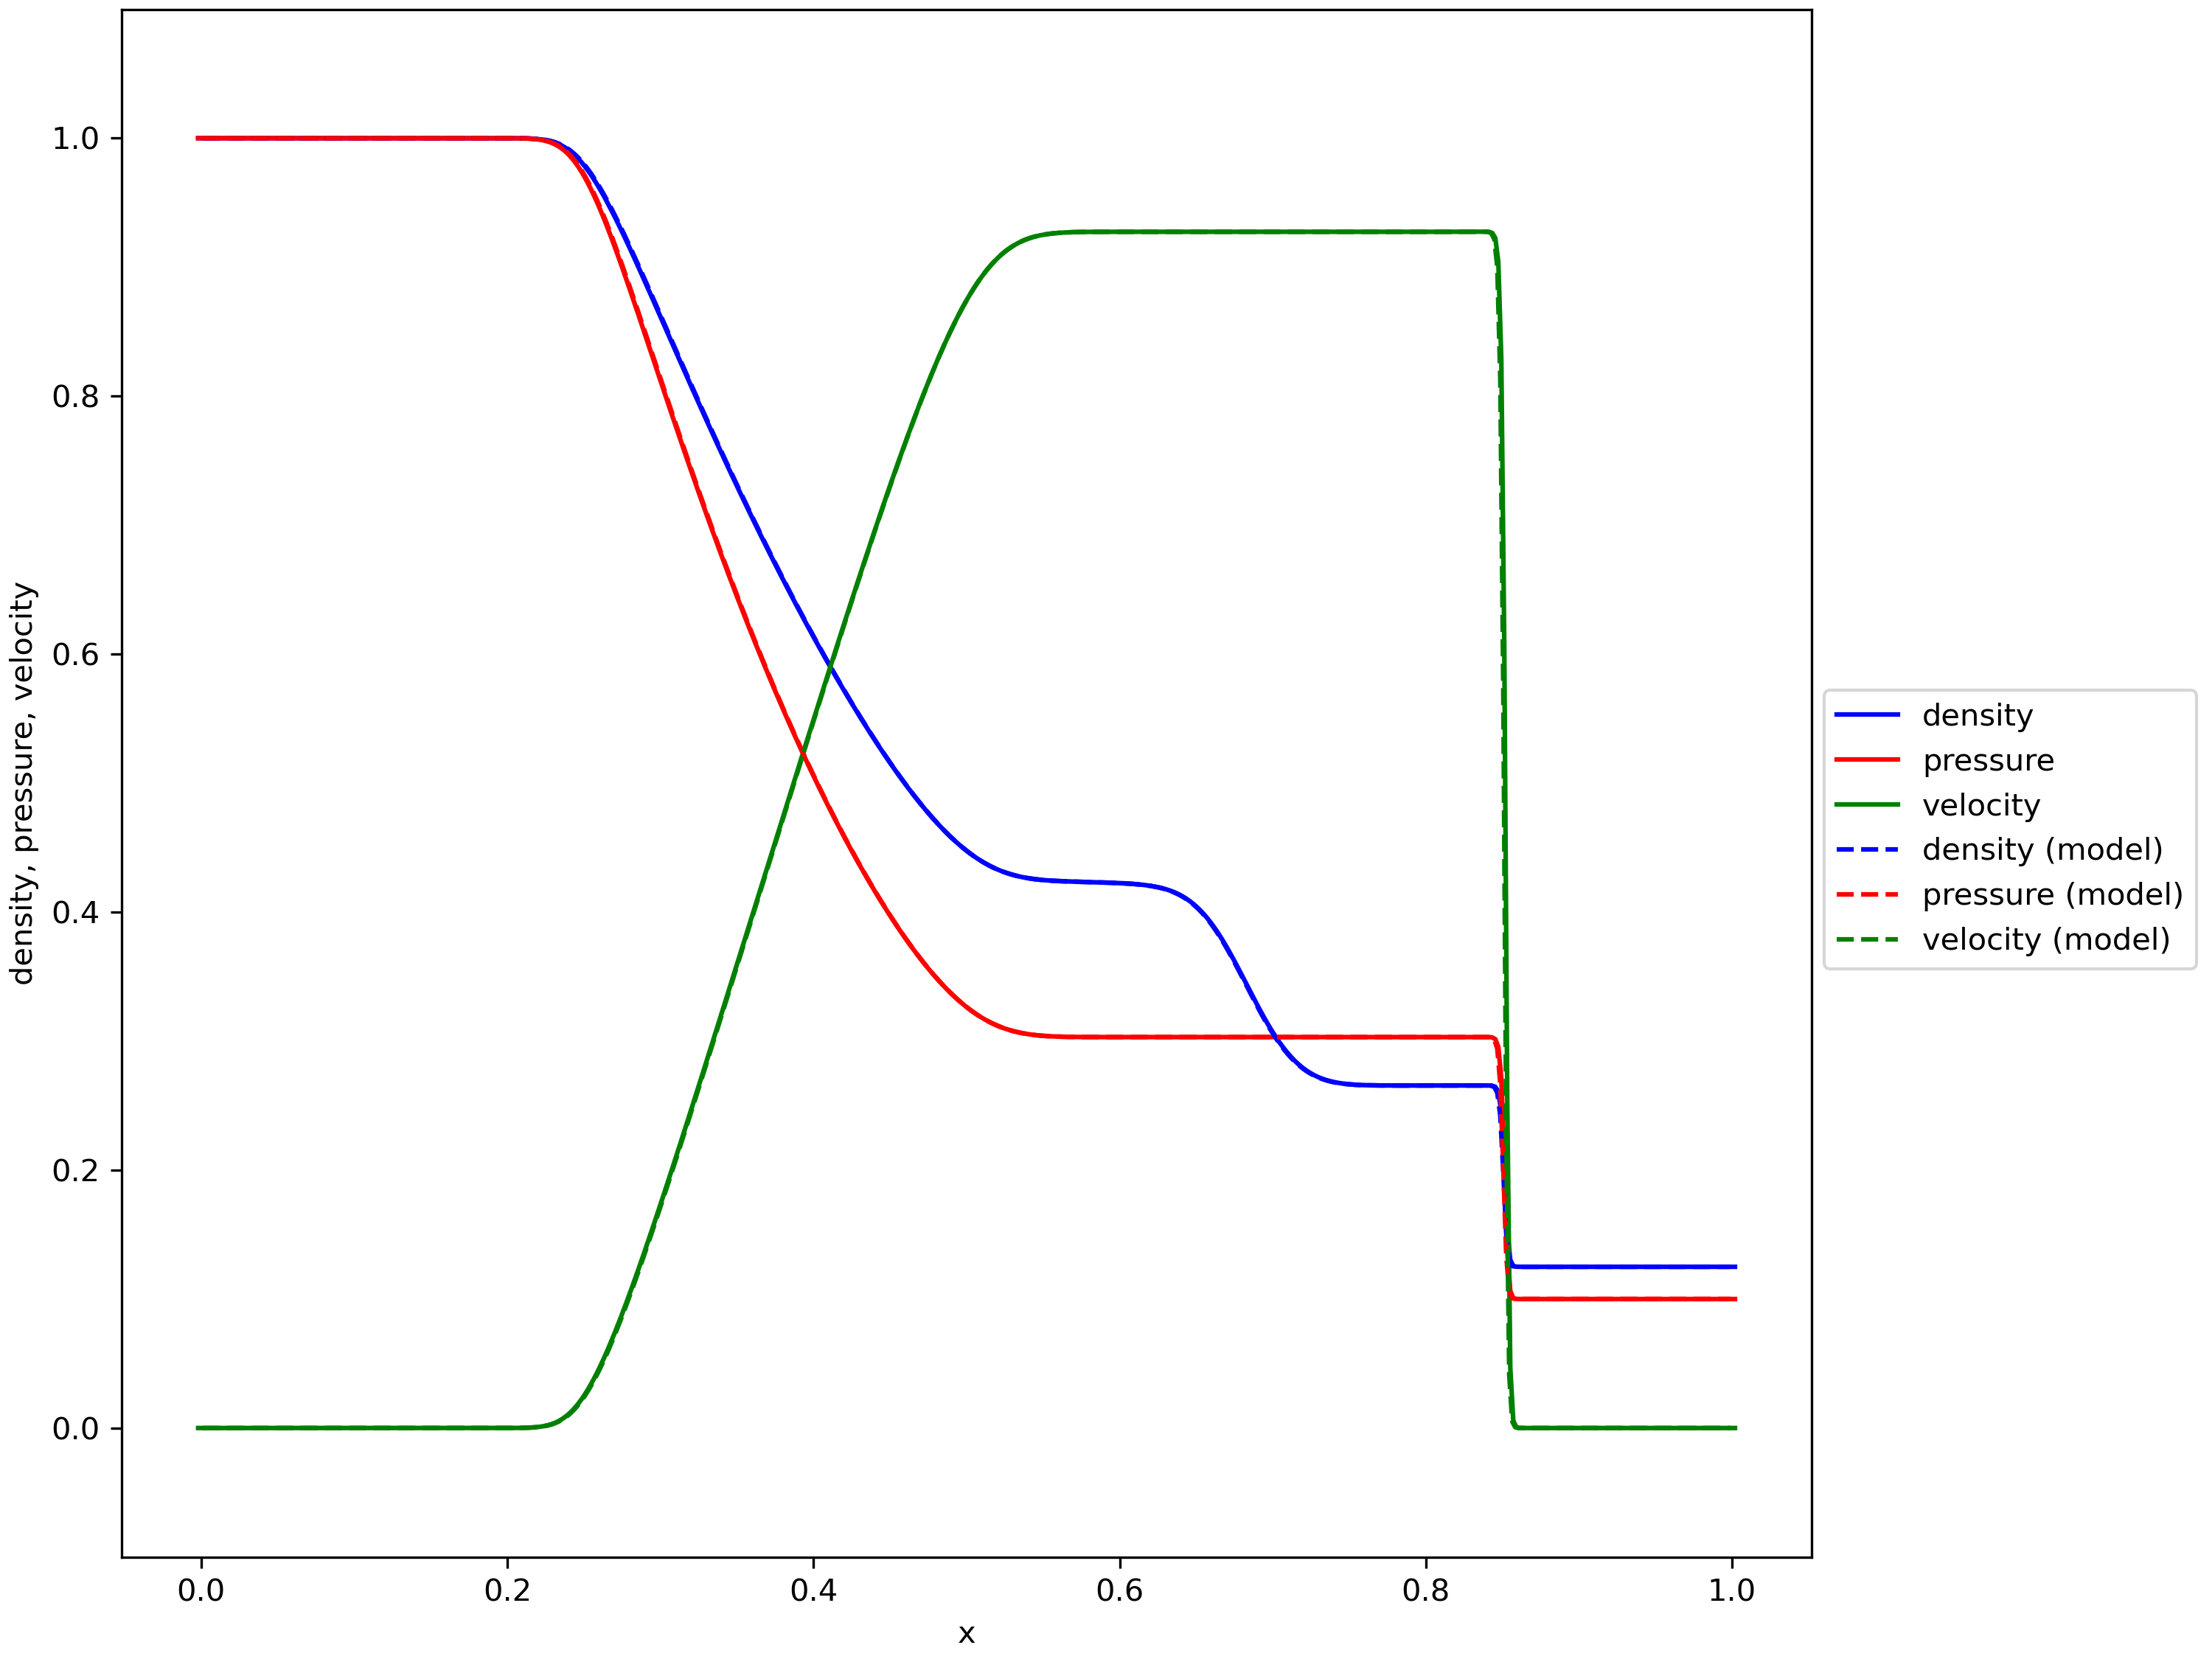
\includegraphics[keepaspectratio]{images/1d_flat_euler.png}}

}

\subcaption{\label{fig-euler_end}Euler time-stepping and flat
reconstruction}

\end{minipage}%
%
\begin{minipage}{0.50\linewidth}

\centering{

\pandocbounded{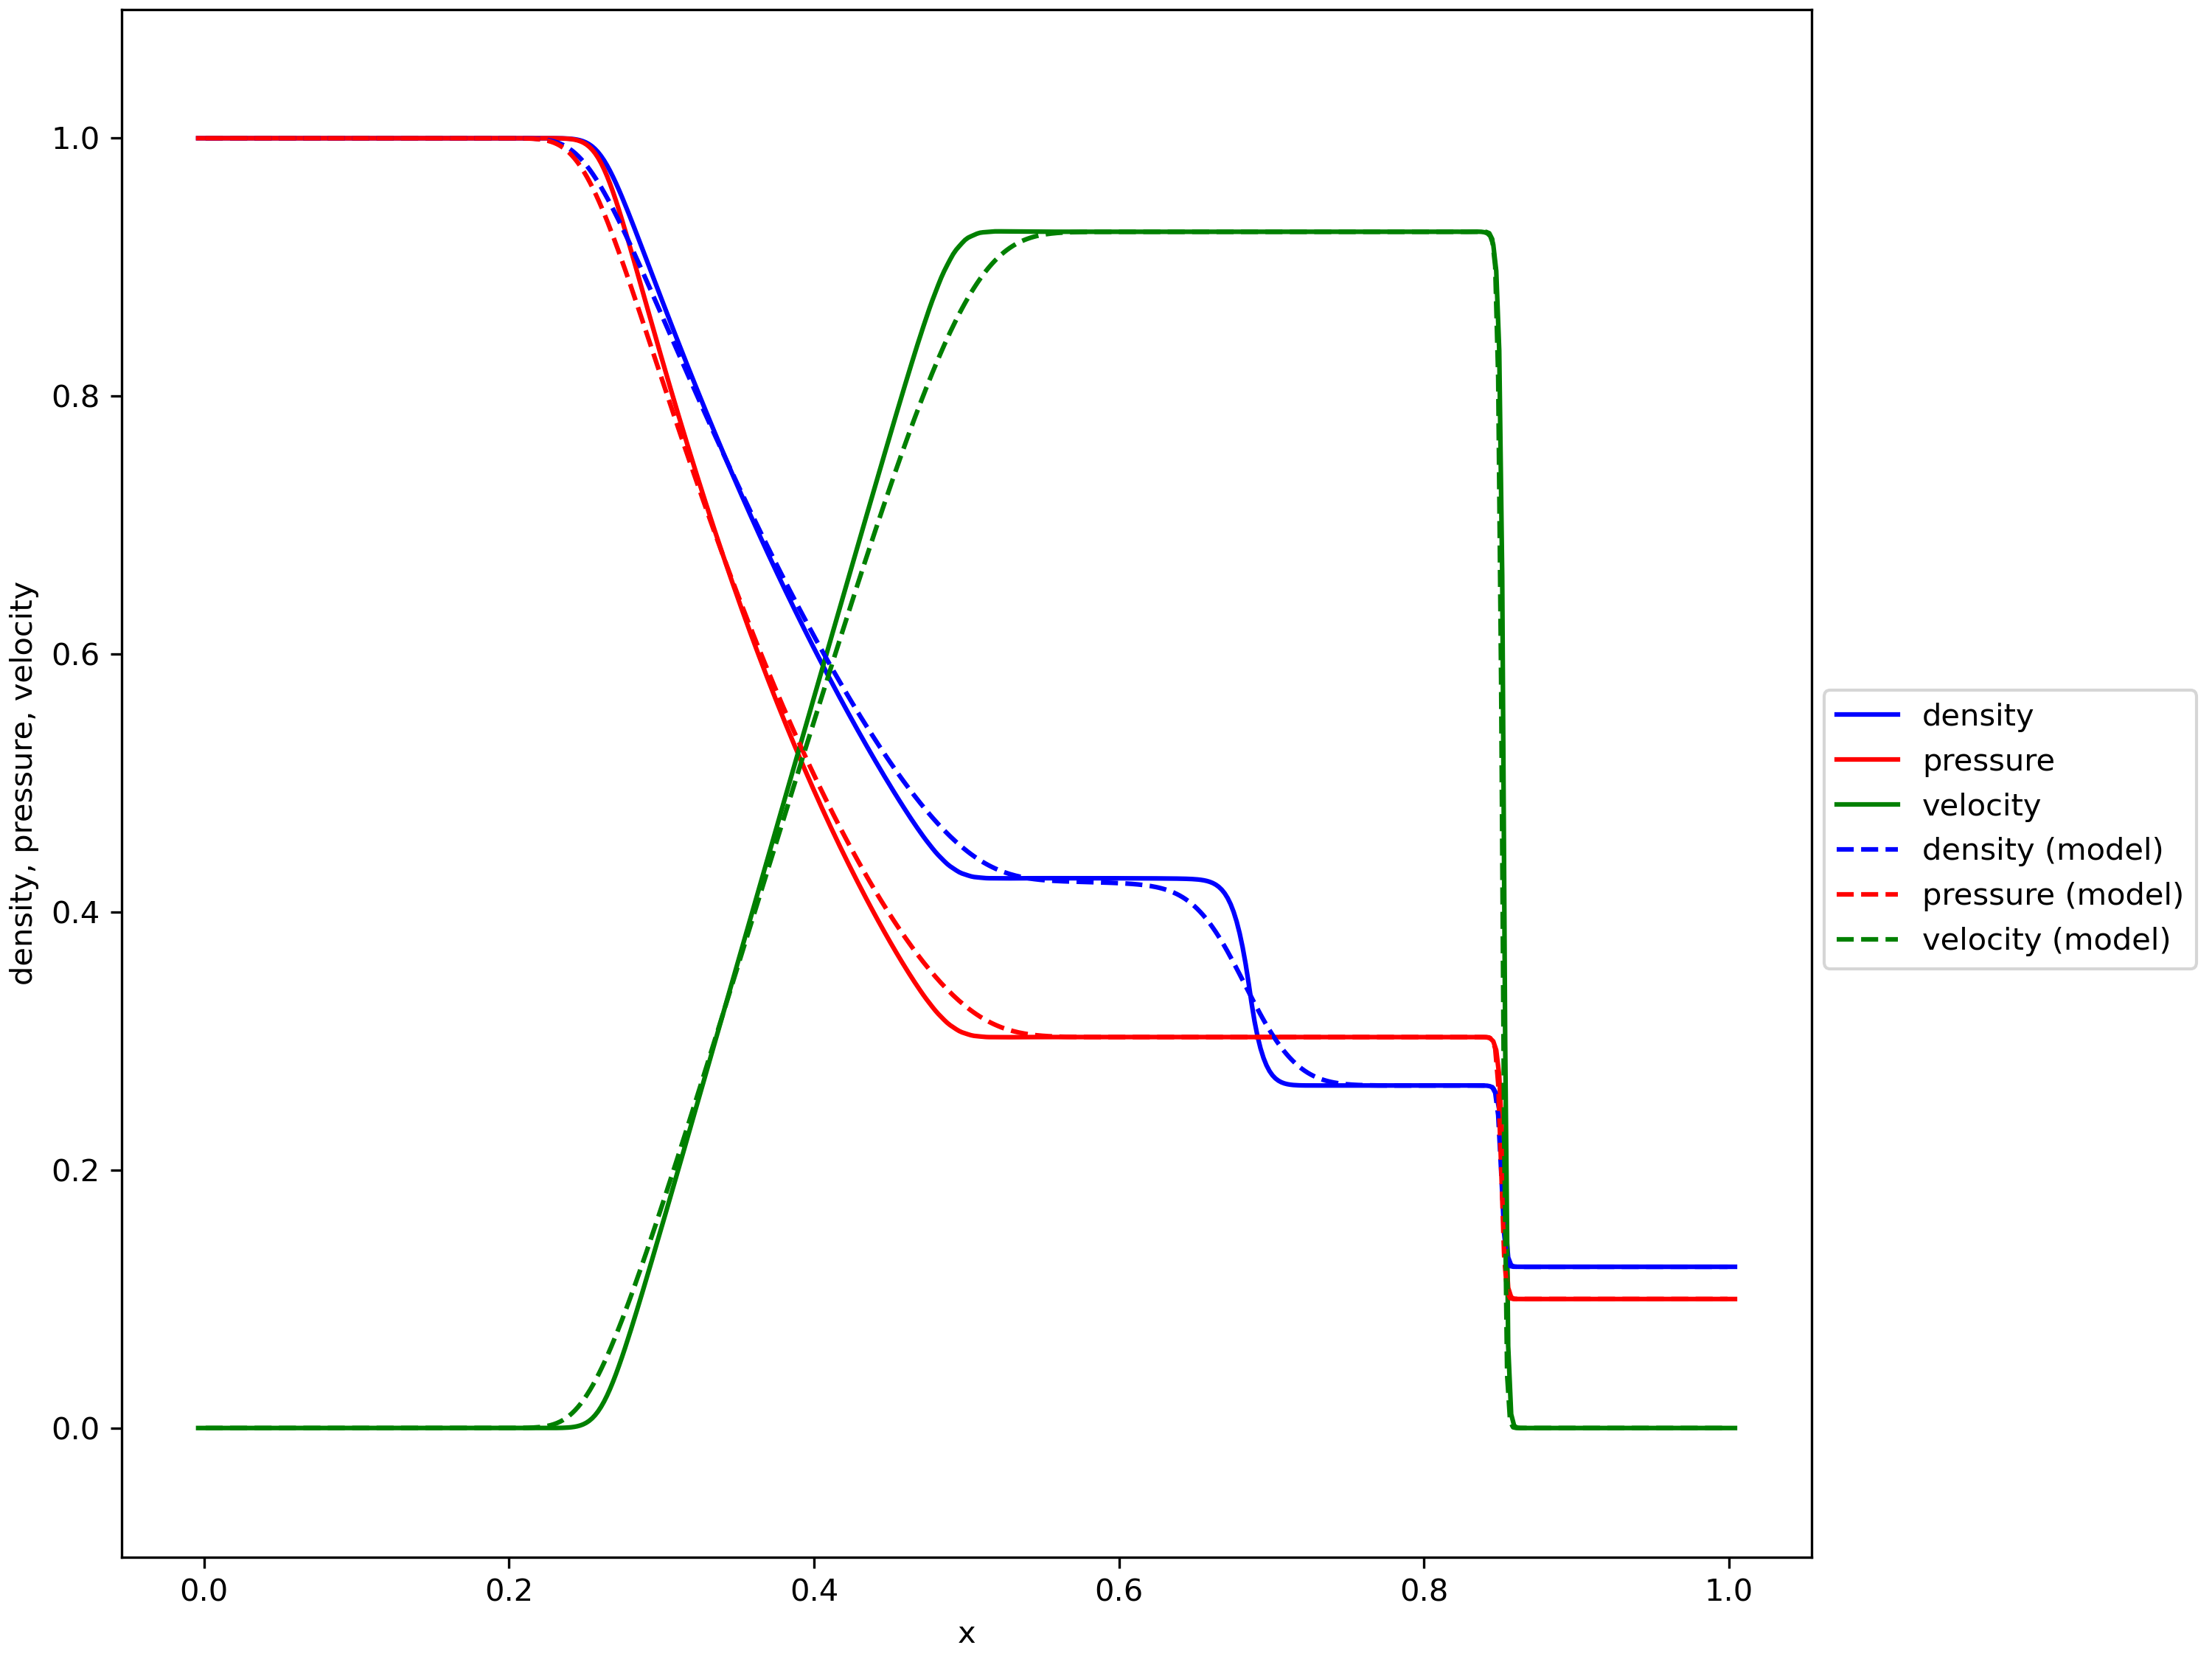
\includegraphics[keepaspectratio]{images/1d_linear_rk4.png}}

}

\subcaption{\label{fig-rk4_end}4\textsuperscript{th} order Runge-Kutta
time-stepping and linear reconstruction}

\end{minipage}%

\caption{\label{fig-shock-tube}Comparison of shock tube simulation
results using various methods.}

\end{figure}%

Given that I was able to recreate the model solution I moved on to the
2D simulations.

\section{2D Problems}\label{d-problems}

\subsection{Blast Wave Example}\label{blast-wave-example}

The first simulation was the Blast Wave problem described in the
detailed project instructions. I changed the problem parameters to be:

\begin{itemize}
\tightlist
\item
  \(-0.5<x<0.5\), \(-0.75<y<0.75\)
\item
  Resolution: \(400 \times 600\)
\item
  Boundary conditions are reciprocal everywhere.
\end{itemize}

These changes were motivated by the Athena Code Test ``Spherical Blast
Wave'' example. I wanted to compare the blast wave example to the Athena
example however there were issues with that which are discussed in
Section~\ref{sec-blast-ring}. If the boundary conditions were
``outflow'' we would not get complex interactions between the waves in
the fluid and the blast would only spread out. As well by changing the
dimensions of \(x\) and \(y\) this leads to differences between the
vertical and horizontal directions.

\begin{figure}

\begin{minipage}{0.33\linewidth}

\centering{

\pandocbounded{
\includegraphics[keepaspectratio]{images/bw_init.png}}

}

\subcaption{\label{fig-blast-wave-init}Initial conditions of the blast
wave}

\end{minipage}%
%
\begin{minipage}{0.33\linewidth}

\centering{

\pandocbounded{
\includegraphics[keepaspectratio]{images/bw_02.png}}

}

\subcaption{\label{fig-blast-wave-02}Blast wave simulation at 0.2
seconds}

\end{minipage}%
%
\begin{minipage}{0.33\linewidth}

\centering{

\pandocbounded{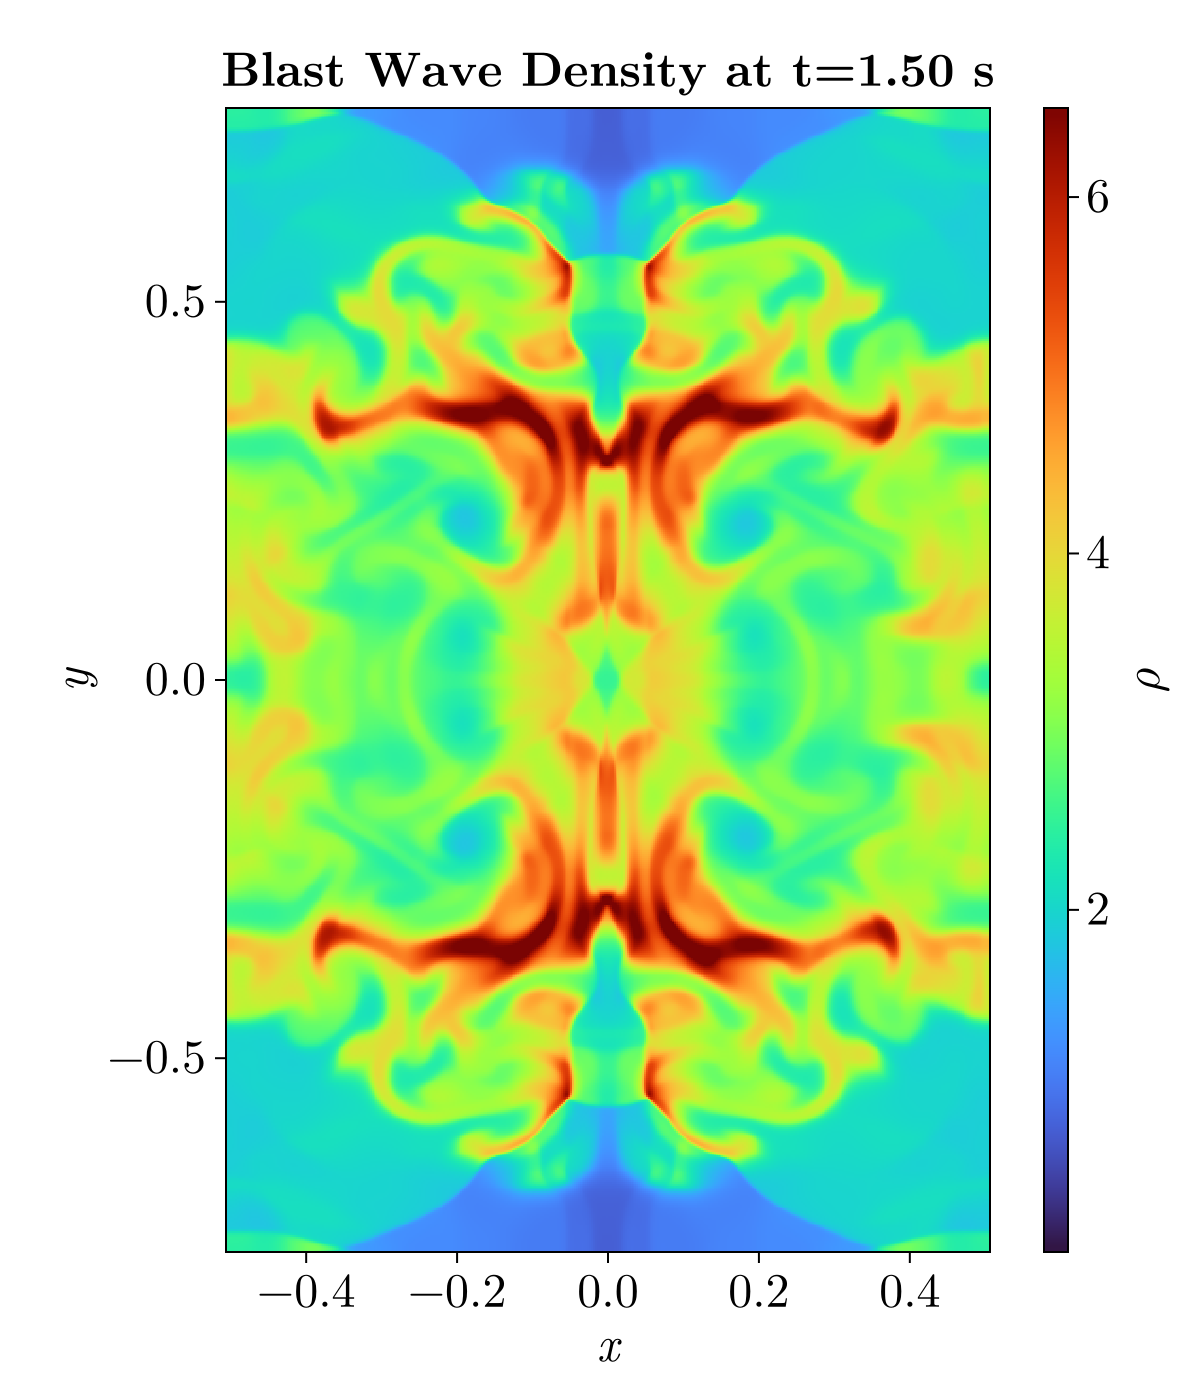
\includegraphics[keepaspectratio]{images/bw_final.png}}

}

\subcaption{\label{fig-blast-wave-end}Blast wave simulation at 1.5
seconds}

\end{minipage}%

\caption{\label{fig-blast-wave-time}The blast wave simulation at various
times.}

\end{figure}%

\subsubsection{Plotting Method}\label{plotting-method}

I created \texttt{plot\_2d.py} by copying \texttt{plot\_1d.py} and
modifying it. First by adding in multiple subplots that showed the
different variables. This was a useful method to ensure that the initial
conditions of the problem were set correctly. I used \texttt{pcolormesh}
to display the images as I am more familiar with that plotting method
than \texttt{imshow}. However, eventually I switched over to plotting in
Julia when making the animations. Julia provides some very useful
plotting features for videos as discussed in Section~\ref{sec-anim}

\subsection{Custom Problems}\label{custom-problems}

Another change that I made was to save the data and plots based on the
\texttt{Name} problem parameter. When switching between the custom
problems there were issues with the new problems overwriting old data
and plots. By using the name parameter in this way each problem is saved
to a unique location. I changed \texttt{output.py} script to use the
\texttt{Name} of the problem as another directory for the output
folders.

I created two custom 2D simulations. The first was a recreation of the
Athena Code Test ``Spherical Blast Wave''. The second was a recreation
of the Athena Code Test ``Kelvin-Helmholtz Instability''.

\subsubsection{Blast Ring}\label{sec-blast-ring}

This problem is a variation on the initial blast wave problem. When
comparing the blast wave Athena Code Test I noticed some discrepancies
between the stated initial conditions and the provided demonstration. As
Figure~\ref{fig-athena-blast-init} shows the initial conditions for the
Athena simulation were not an initial overdensity within \(r<0.1\).

Instead the simulation starts from a ring at \(r=0.1\) with the
overdensity. I was able to implement this by creating a mask around
\(r=0.1\) and setting the overdensity there. After some experimenting I
found that a ring with width \(\Delta r = 0.005\) reasonably recreated
the Athena simulation. Figure~\ref{fig-blast-ring-init} shows this
initial setup.

\begin{figure}

\begin{minipage}{0.50\linewidth}

\centering{

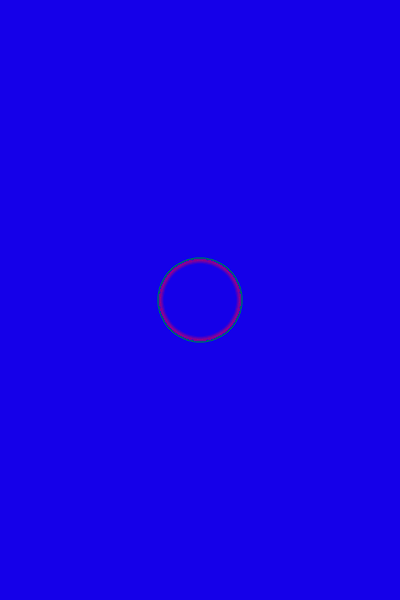
\includegraphics[width=0.7\linewidth,height=\textheight,keepaspectratio]{images/athena_code_tests/hydro-blast-frames/frame_001_delay-0.05s.png}

}

\subcaption{\label{fig-athena-blast-init}Athena Code Test ``Blast Wave''
initial conditions}

\end{minipage}%
%
\begin{minipage}{0.50\linewidth}

\centering{

\pandocbounded{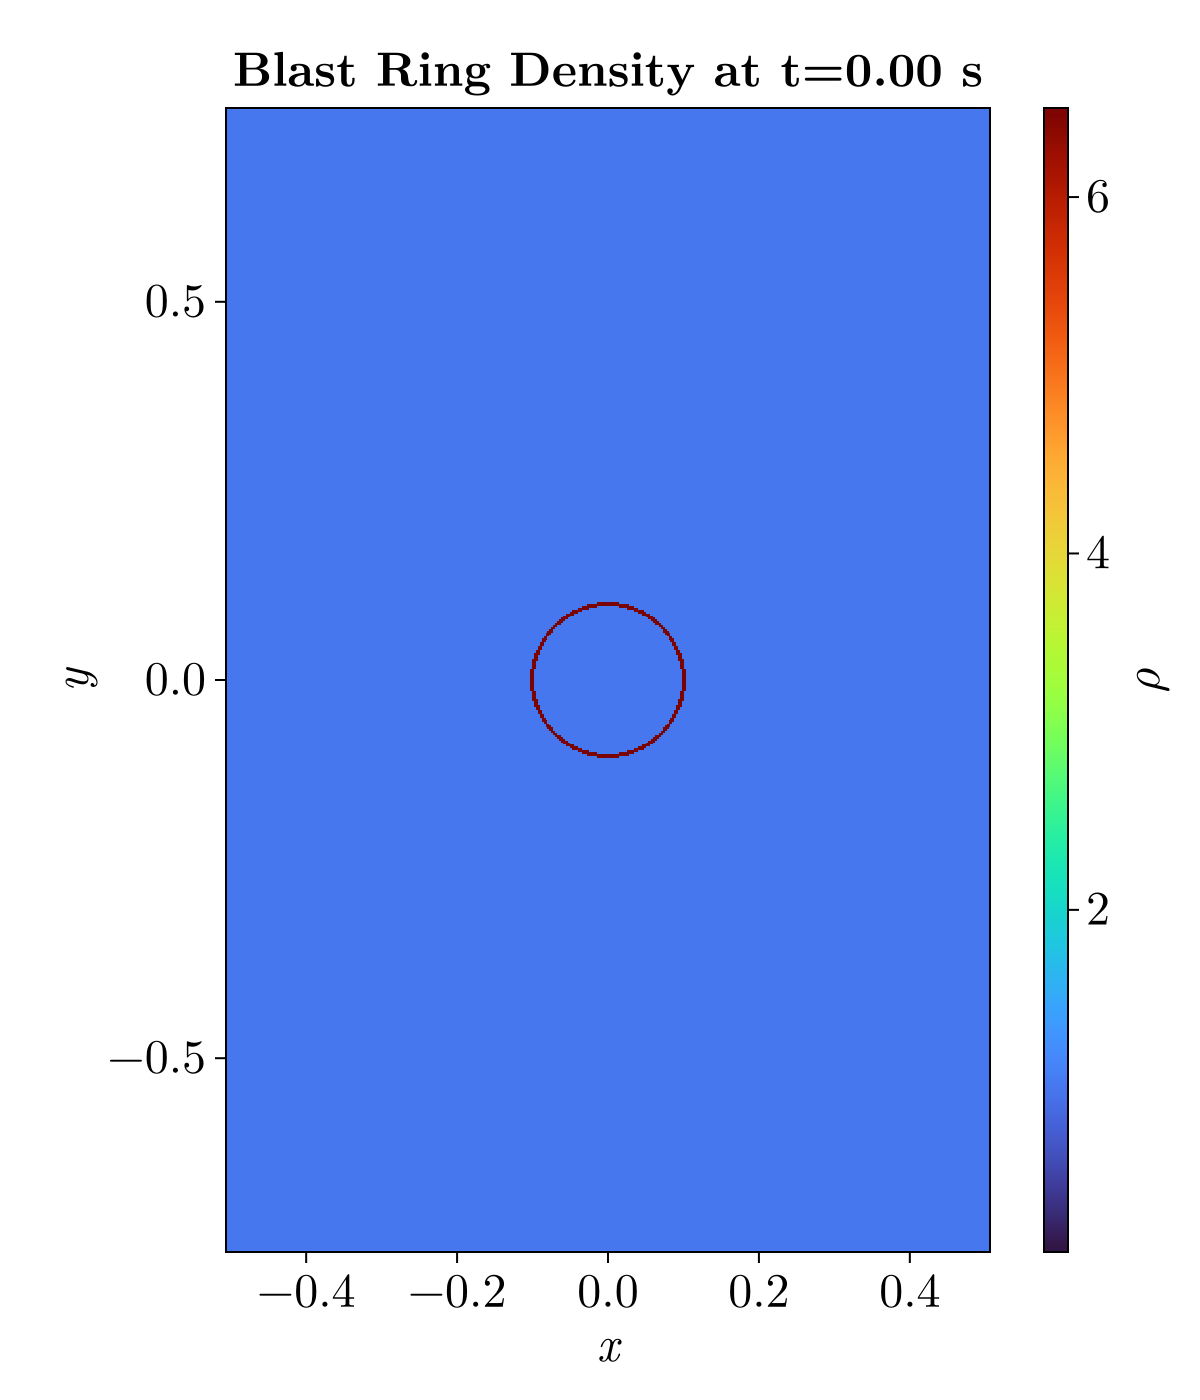
\includegraphics[keepaspectratio]{images/br_init.png}}

}

\subcaption{\label{fig-blast-ring-init}My blast ring initial condition}

\end{minipage}%

\caption{\label{fig-br-compare-init}The initial conditions of the blast
ring simulation.}

\end{figure}%

The main comparison for this problem is the creation of ``fingers''
within the fluid that do not dissipate after creation. As well as the
density being symmetric horizontally and vertically throughout the
simulation.

\begin{figure}

\begin{minipage}{0.50\linewidth}

\centering{

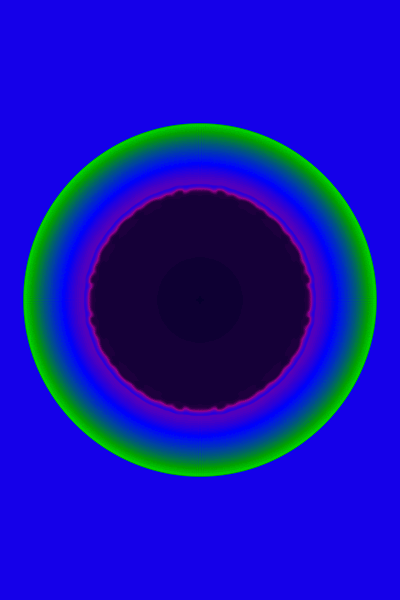
\includegraphics[width=0.7\linewidth,height=\textheight,keepaspectratio]{images/athena_code_tests/hydro-blast-frames/frame_100_delay-0.05s.png}

}

\subcaption{\label{fig-athena-blast-t02}Athena blast wave simulation}

\end{minipage}%
%
\begin{minipage}{0.50\linewidth}

\centering{

\pandocbounded{
\includegraphics[keepaspectratio]{images/br_02.png}}

}

\subcaption{\label{fig-blast-ring-t02}Blast ring simulation}

\end{minipage}%

\caption{\label{fig-br-compare}Comparison of Athena simulation and my
simulation at \(t=0.2\)s.}

\end{figure}%

\subsubsection{Kelvin-Helmholtz}\label{kelvin-helmholtz}

For the second custom problem I decided to look at the Kelvin-Helmholtz
Instability. This was mentioned in the lectures and produced beautiful
videos. The initial conditions I used were based on the Athena Code
Test.

\begin{itemize}
\tightlist
\item
  \(-0.5 < x < 0.5\), \(-0.75 < y < 0.75\)
\item
  Resolution: \(512 \times 512\)
\item
  Pressure: \(2.5\) everywhere
\item
  \(|y| > 0.25\) has density \(1.0\) and \(v_{x}=-0.5\)
\item
  \(|y| < 0.25\) has density \(2.0\) and \(v_{x}=0.5\)
\item
  \(v_{y} = 0.0\) everywhere
\item
  Reciprocal boundary conditions everywhere
\end{itemize}

However with just these initial conditions the instabilities did not
form. I had missed an important line in the initial conditions:

\begin{tcolorbox}[enhanced jigsaw, opacityback=0, left=2mm, titlerule=0mm, breakable, toprule=.15mm, coltitle=black, leftrule=.75mm, colframe=quarto-callout-note-color-frame, opacitybacktitle=0.6, bottomrule=.15mm, bottomtitle=1mm, toptitle=1mm, colbacktitle=quarto-callout-note-color!10!white, title=\textcolor{quarto-callout-note-color}{\faInfo}\hspace{0.5em}{Kelvin-Helmholtz Initial Condition}, arc=.35mm, rightrule=.15mm, colback=white]

To seed the instability, we add random numbers to both the x- and
y-components of the velocity with peak-to-peak amplitude of \(0.01\).

\end{tcolorbox}

Without these random velocities the instabilities did not form and the
flow continued smoothly. Figure~\ref{fig-kh} shows the initial
conditions of the Kelvin-Helmholtz Instability. While it is not visible
in the \(v_{x}\) subplot the \(v_{y}\) subplot shows the initial random
velocities.

\begin{figure}

\centering{

\pandocbounded{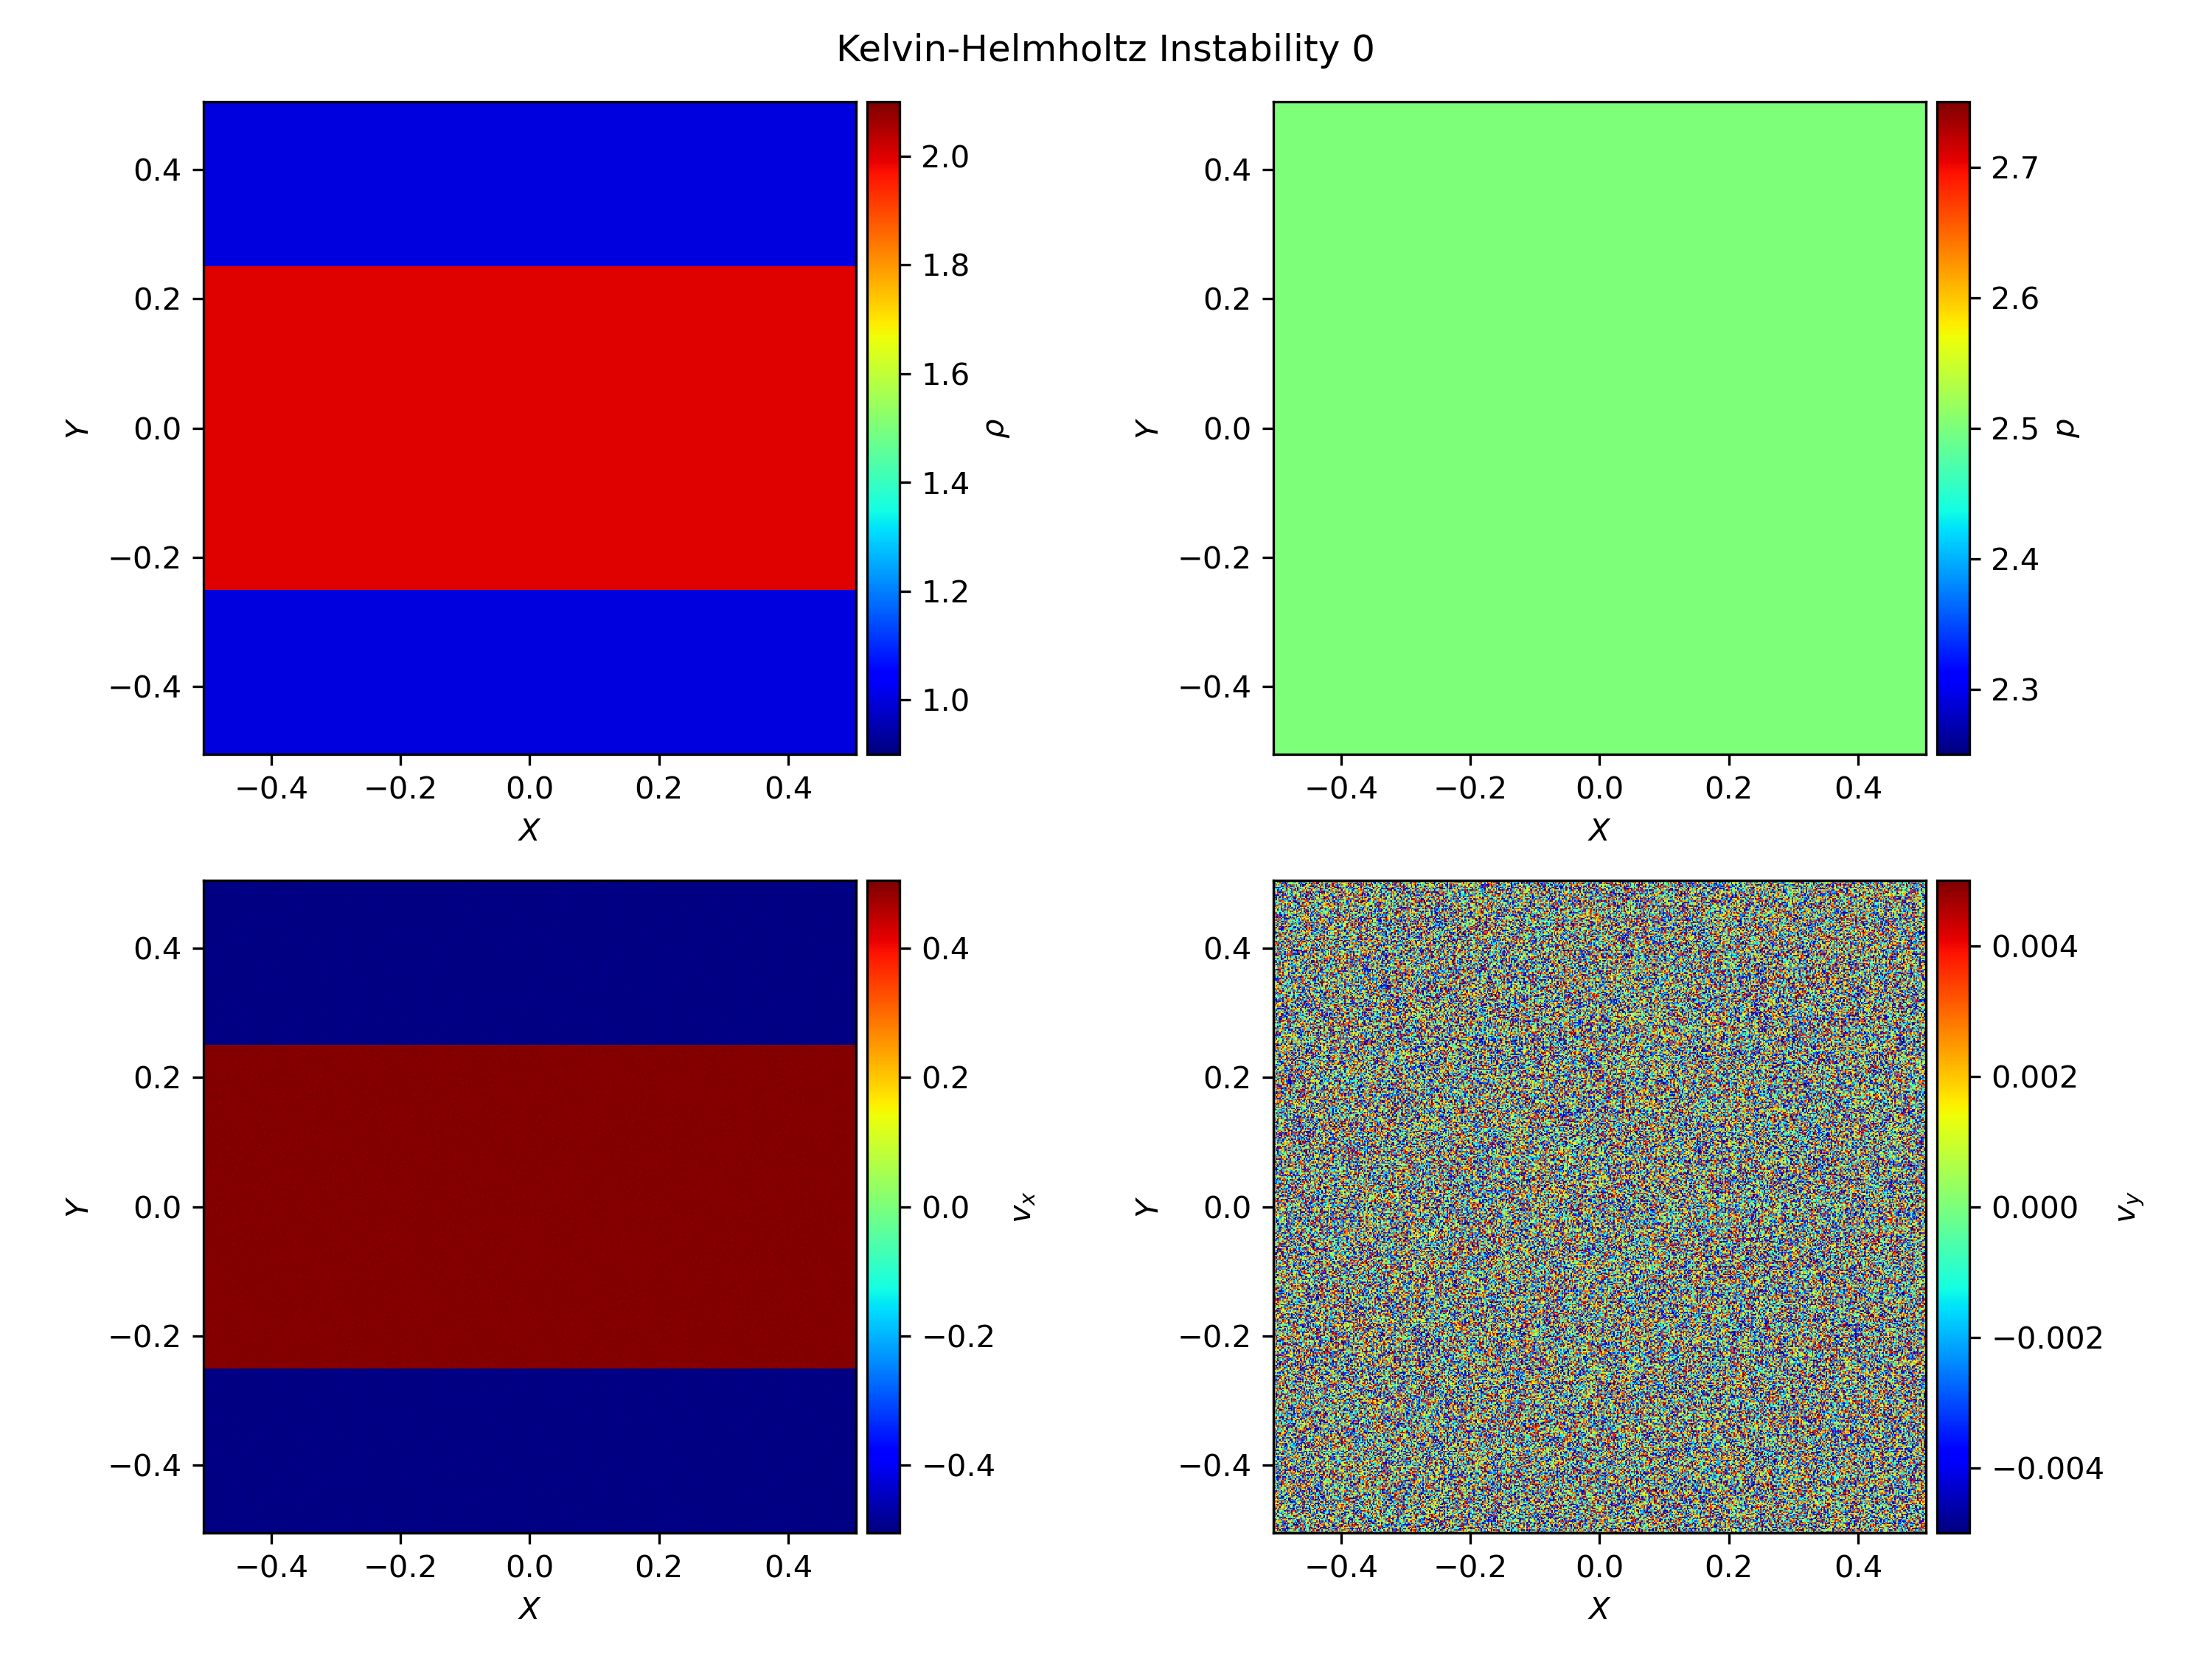
\includegraphics[keepaspectratio]{images/kh_0000.png}}

}

\caption{\label{fig-kh}Initial conditions of the Kelvin-Helmholtz
Instability simulation.}

\end{figure}%

Initially I ran this simulation for a simulation time of \(t=1.0\)s.
However the instabilities were just beginning to form, unlike in the
Athena code test where the instabilities were already visible at one
second, see Figure~\ref{fig-kh-compare}.

\begin{figure}

\begin{minipage}{0.50\linewidth}

\centering{


\includegraphics[width=0.85\linewidth,height=\textheight,keepaspectratio]{images/athena_code_tests/khmovie-frames/frame_100_delay-0.05s.png}

}

\subcaption{\label{fig-athena-kh-1}Athena Kelvin-Helmholtz Instability
simulation}

\end{minipage}%
%
\begin{minipage}{0.50\linewidth}

\centering{

\pandocbounded{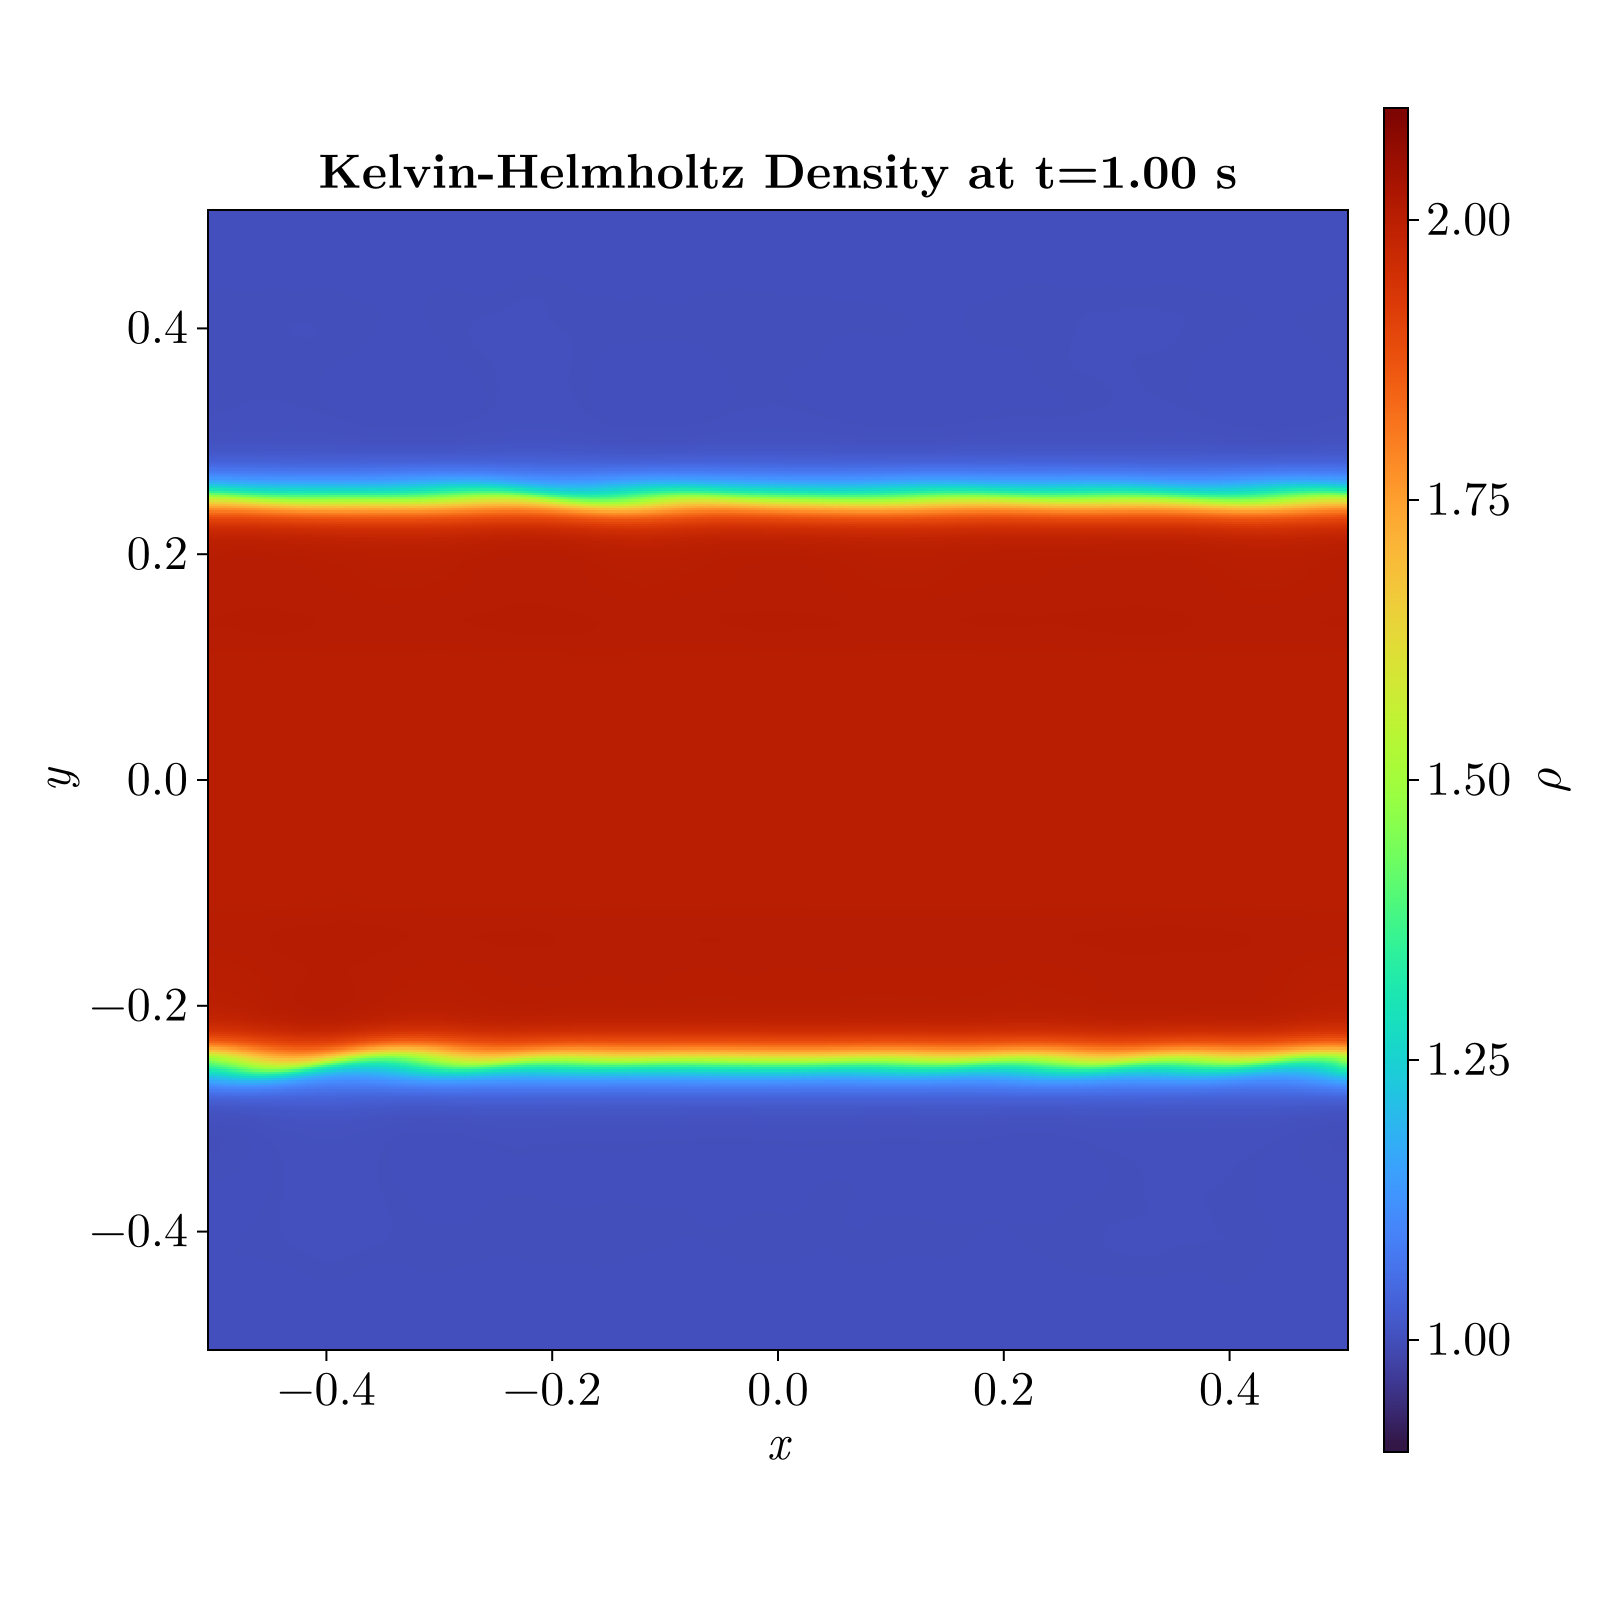
\includegraphics[keepaspectratio]{images/kh_1_plot.png}}

}

\subcaption{\label{fig-kh-t1}My Kelvin-Helmholtz Instability}

\end{minipage}%

\caption{\label{fig-kh-compare}Comparison of Kelvin-Helmholtz
Simulations at \(t=1.0\)s of simulation time.}

\end{figure}%

But as it seemed the instabilities were forming I decided to increase
the max time parameter to five seconds to match the Athena simulation.
Increasing the simulation time made the simulation take approximately
2.5 hours, using the linear reconstruction method and RK4.
Figure~\ref{fig-kh-t2} shows the instabilities forming at two seconds.

\begin{figure}

\centering{

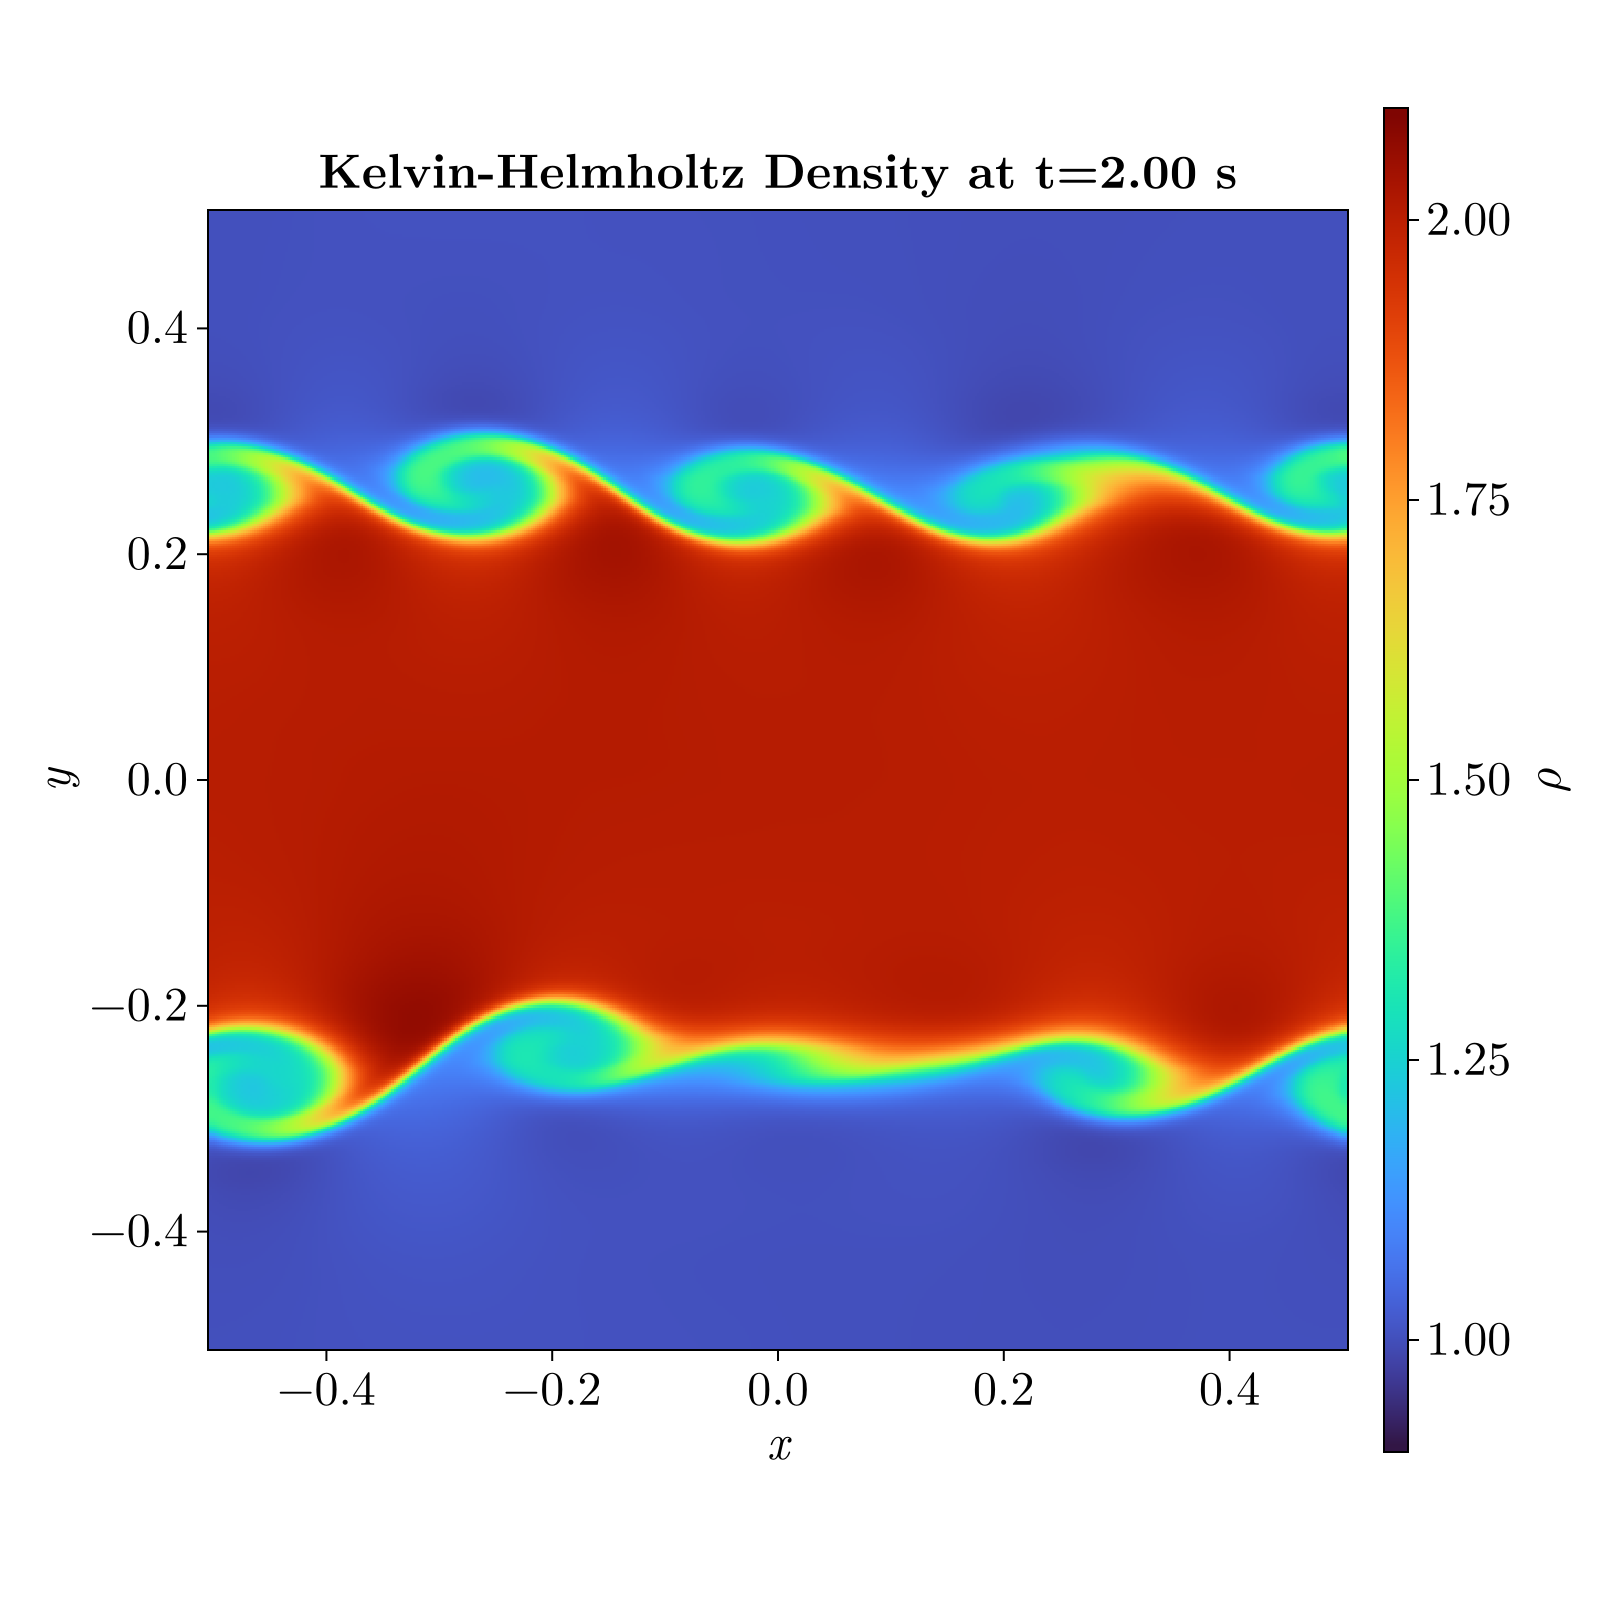
\includegraphics[width=0.5\linewidth,height=\textheight,keepaspectratio]{images/kh_2_plot.png}

}

\caption{\label{fig-kh-t2}Kelvin-Helmholtz Instability simulation at two
seconds.}

\end{figure}%

The simulation does achieve the expected instabilities. However when
comparing to the Athena code test there is a lack of detail. There are a
few potential reasons for these differences. The main one comes from
Athena using more advanced solvers that preserve those small details.
The linear reconstruction method is not able to retain those small
vortices. As well Athena used the ``hllc'' Riemann solver while this
simulation used ``hll''. From what I have seen the hllc solver utilizes
a more accurate model of the waves which retains that extra detail.

\section{Animation}\label{sec-anim}

I attempted many methods for animating the results:

\begin{itemize}
\tightlist
\item
  FFmpeg to convert the generated plots to a .mp4 file.
\item
  yt-project to make the plots and then stitch them together with
  FFmpeg.
\item
  \texttt{matplotlib.animation} library to automatically make the video
\item
  julia plotting as making animations is very easy

  \begin{itemize}
  \tightlist
  \item
    animating with the \texttt{@animate} macro using \texttt{Plots}
  \item
    animating using \texttt{Observables} and \texttt{CairoMakie}
  \end{itemize}
\end{itemize}

The method that I eventually settled on was to make the animations in
Julia using the CairoMakie package. This package makes use of
\texttt{Observables} that are variables that julia monitors and uses the
GPU to change in place. This method make videos faster than the standard
method from matplotlib or making the frames individually and stitching
them together.

At first I just plotted the densities using a heatmap to ensure that the
videos were generating properly. Once that was confirmed to work I
included the other variables pressure, \(p\), and the velocity fields.

The velocity animation took the longest to make work. Initially I wanted
to use streamlines to show the velocity flow. However when attempting
this in both python and julia there were a few issues. The main one
being that the streamlines between frames were not consistent. So the
video did not provide an understanding of how the flow changes over
time. I changed from using streamlines to using \texttt{arrows2d} which
is equivalent to matplotlibs \texttt{quiver} function. This shows the
velocity field over time and by sampling specific points within the
velocity field it was consistent.

The pressure was made using the same heatmap method as for the density
but with a different colorscale. At first I set the pressure colorscale
based on the density colorscale and dividing by the value of \(\gamma\)
used in that simulation. This generally worked but did not provide all
the detail I wanted, so eventually I just tried different values to
reveal more detail.

For the animation of the Kelvin-Helmholtz problem I wanted to see the
formation of larger vortices so I increased the simulation time to 10
seconds. This took approximately six hours to run using linear
reconstruction and RK4. The vortices did grow over time as
Figure~\ref{fig-kh-final} shows the last frame of the simulation.

\section{Conclusion}\label{conclusion}

This was a interesting project allowing us to dive deeper into
computational fluid dynamics (CFD). CFD is a topic I have wanted to
explore for a while but have not had the chance to before. It was useful
to focus on just a few aspects of the code but being able to see how the
various parts of the simulation fit together. I have certainly gained a
deeper understanding and appreciation of what it takes to develop a
computational fluid dynamics system. As well it was fun making my own
simulations and producing beautiful plots and movies.

\begin{figure}

\centering{

\pandocbounded{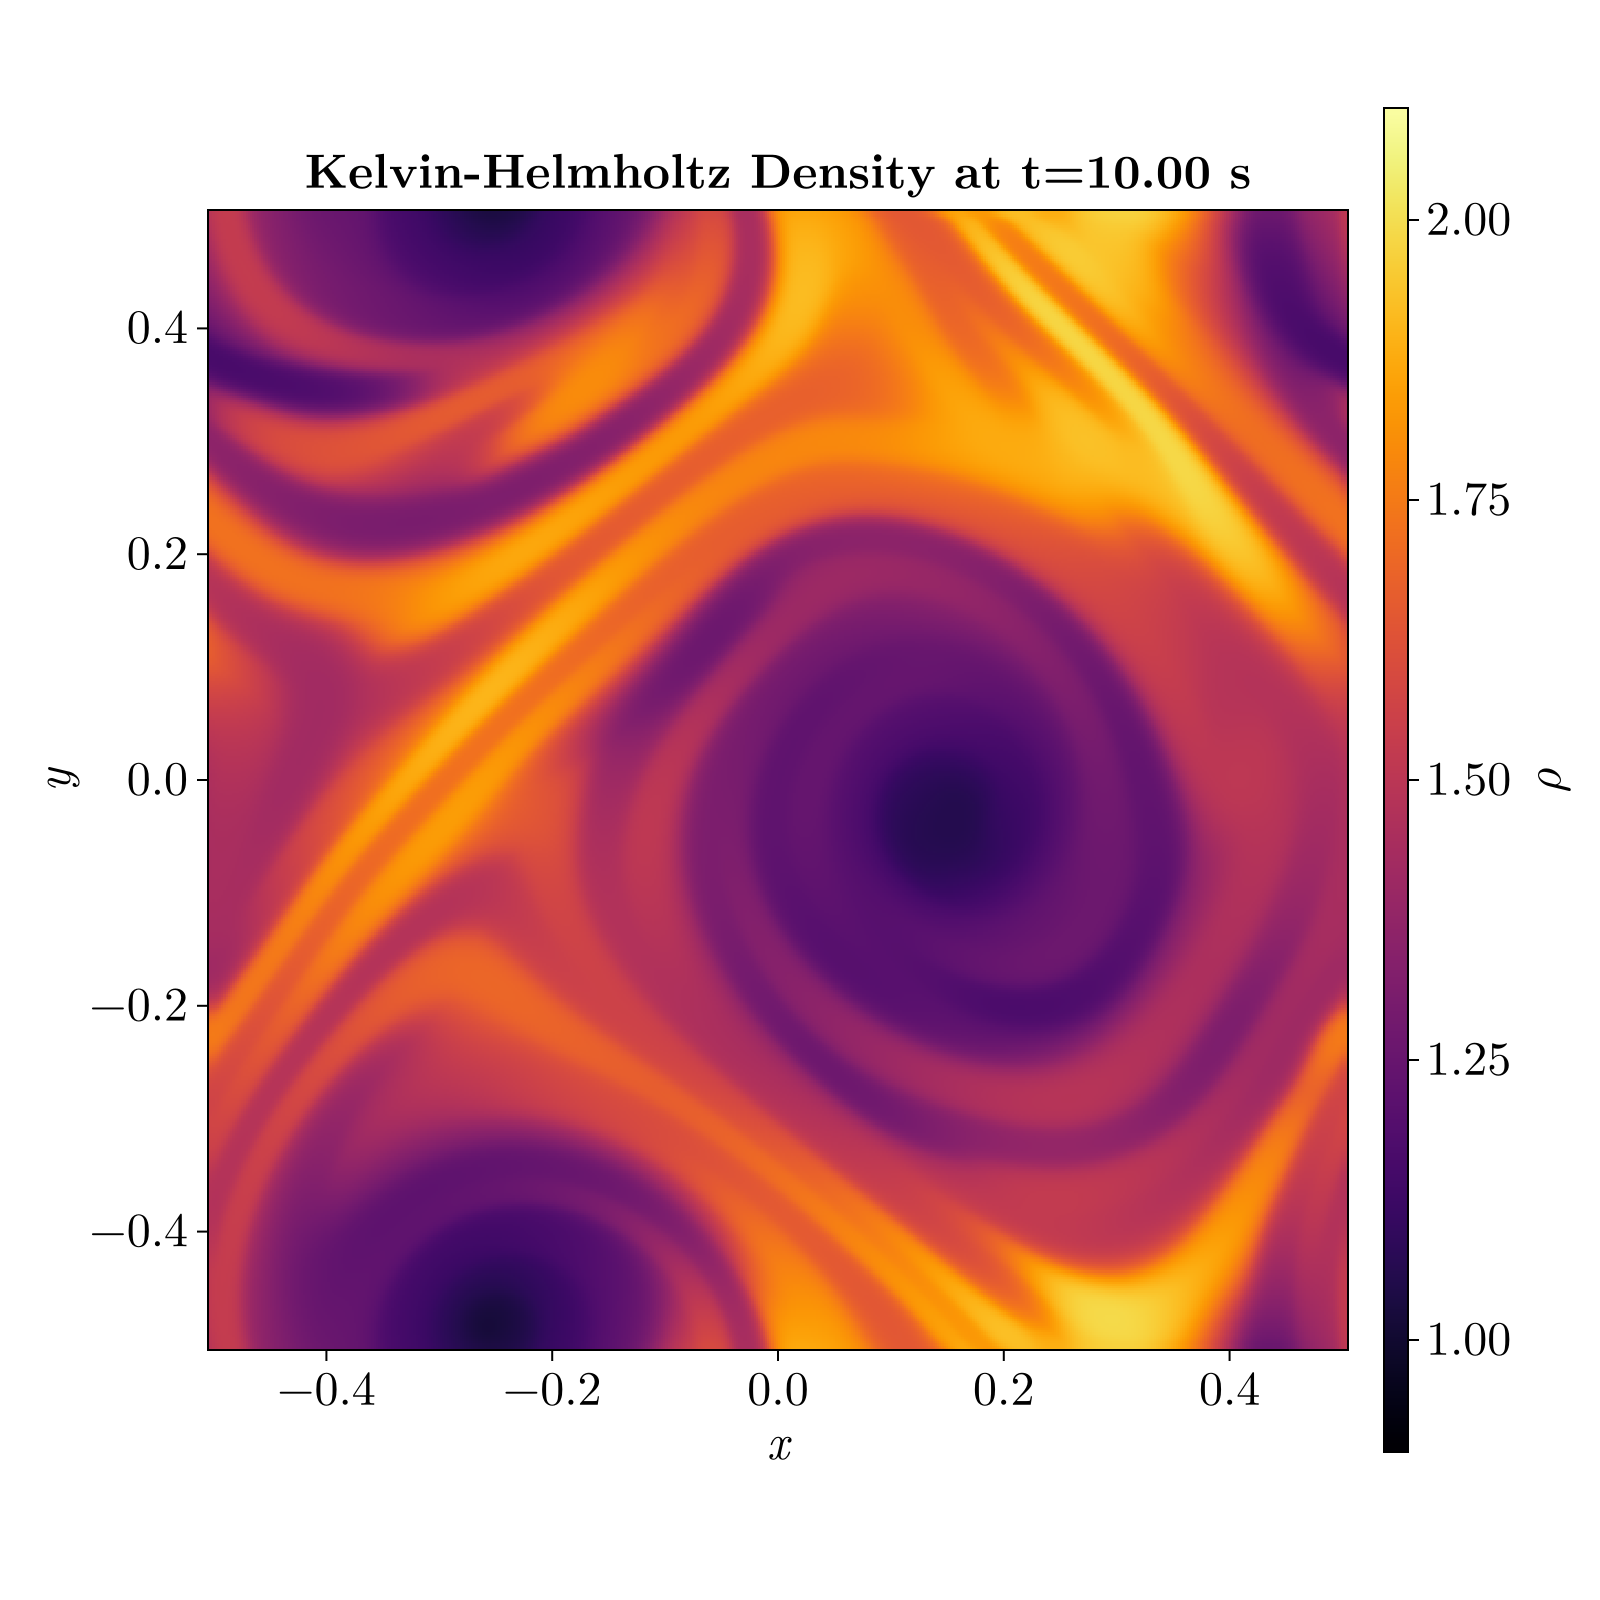
\includegraphics[keepaspectratio]{images/kh_final_plot.png}}

}

\caption{\label{fig-kh-final}Kelvin-Helmholtz Instability simulation at
10 seconds.}

\end{figure}%




\end{document}
